%!TEX root = ../report.tex
\section{Hopf bifurcation}

Continuing on the upper branch of the pitchfork, we compute (at most) 6 of the eigenvalues closest to the origin after a few steps in $Re.$ After a while we find that a conjugate eigenpair crosses the imaginary axis, which indicates a Hopf bifurcation is nearby. The movement of the eigenvalues is visualized in Figure~\ref{fig:eigenpair_crossing_imag}.

\begin{figure}[h]
  \caption{A conjugate eigenpair crossing the imaginary axis.}
  \label{fig:eigenpair_crossing_imag}
  \centerline{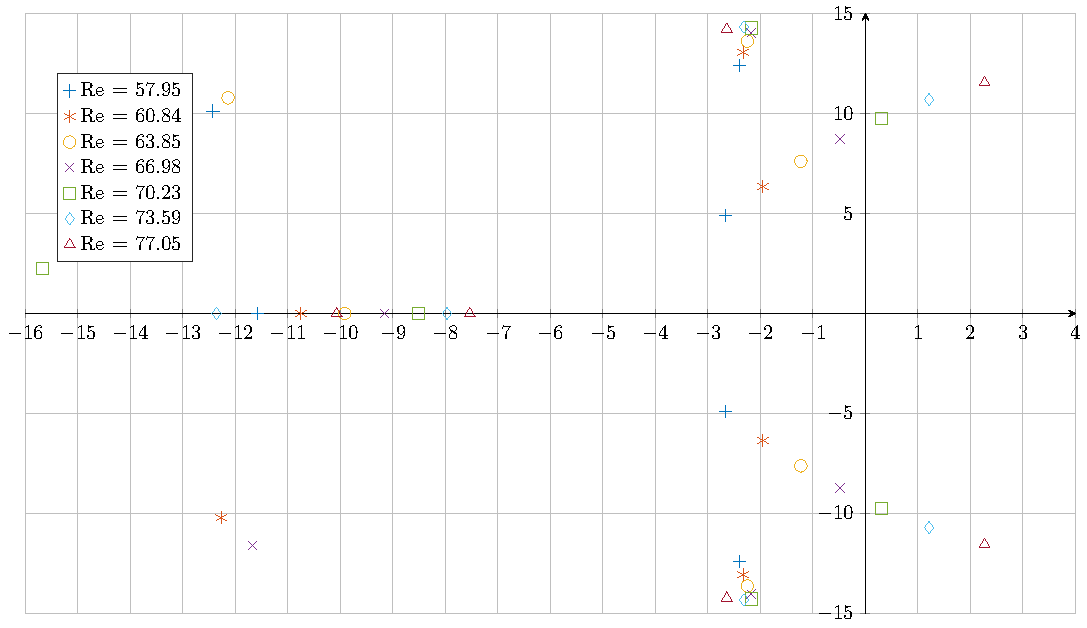
\includegraphics[width=\textwidth]{images/eigenwaarden_hopf.pdf}}
\end{figure}

We apply the secant procedure to compute the value of $Re$ where the first eigenvalue $\lambda$ is completely imaginary, i.e. $\Re(\lambda) = 0.$ We find that the Hopf bifurcation is located at $Re_H \approx 68.9781.$ The conjugate eigenpair is $$\lambda_\pm \approx \pm 9.372i.$$

The real part of the corresponding eigenvectors is shown in Figure~\ref{fig:eigenfunction}.

\begin{figure}
  \caption{Real part of the eigenfunction corresponding to the eigenvalues $\lambda_\pm \approx \pm 9.372i$}
  \label{fig:eigenfunction}
  \centerline{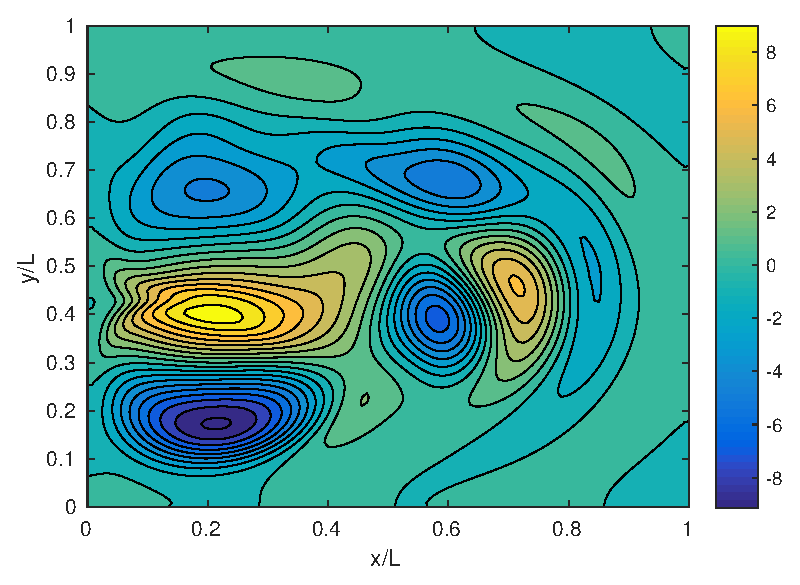
\includegraphics[width=\textwidth]{images/eigenvector_bij_hopf_reele_deel.eps}}
\end{figure}